\documentclass[10pt]{article}

\usepackage[bottom]{footmisc}

\usepackage{xcolor}

\usepackage{amsthm}
\usepackage{amssymb}
\usepackage{amsmath}

\usepackage{mathtools}

\usepackage{hyperref}

\usepackage{caption}
\usepackage{subcaption}

\usepackage{xepersian}

\settextfont{Adobe Arabic}
\setlatintextfont[Scale= 0.85]{Times New Roman}

%{t-size} {mt-size} {s-size} {ss-size}
\DeclareMathSizes{10}{8}{6}{4}

\renewcommand{\qedsymbol}{\rule{0.2cm}{0.2cm}}

\theoremstyle{definition}
\newtheorem*{definition}{تعریف}

\theoremstyle{lemma}
\newtheorem*{lemma}{لم}

\theoremstyle{theorem}
\newtheorem*{theorem}{قضیه}

\theoremstyle{remark}
\newtheorem*{remark}{ \textbf{ملاحضه} }

\newcommand{\tEng}[1]{ \lr{\textsc{#1}} }


\title{گزارش پروژه‌ی شبیه سازی 2 احتمال}
\author{آریا ادیبی ۹۲۱۱۰۴۷۶}
\date{}

\definecolor{darkishBlue}{RGB}{27, 71, 188}

\hypersetup{
	colorlinks= true,
	linkcolor= darkishBlue,
%	anchorcolor= black,
	citecolor= black,
%	filecolor= cyan,
%	menucolor= red,
%	runcolor= cyan,
	urlcolor= darkishBlue,
%	allcolors= black
}

\setcounter{secnumdepth}{0}

\begin{document}
	\maketitle
	
	 قبل از هر چیز ذکر چند نکته ضروری است:
	 \begin{itemize}
	 	\item
	 	اسمی که خواسته شده بود برای فایل‌های کد خود بگذاریم اسمی استاندارد نبود و من به دلیل
	 	این که مشکلی پیش نیاید یا حداقل «اخطار» این موضوع را نبینم این اسم را به
	 	\lr{qi\_studentNumber.m}
	 	تغییر دادم که در آن
	 	\lr{i}
	 	شماره‌ی پرسش است.
	 	%%%%
	 	\item
	 	کامپیوتر من قدرت نسبتاً زیادی دارد از این رو نمی‌دانستم که شمار آزمایش‌ها یا متغیر‌های 
	 	مربوط دیگر را چقدر بگذارم که از کامپوتر مقصد زمان زیادی نگیرد. از این رو در هر کد 
	 	قسمتی به نام
	 	\lr{Initialization}
	 	قرار گرفته که بتوان تمامی متغیر‌های لازم پرسش را به مقدار دلخواه عوض کرد. این انعطاف
	 	بیشتری هم به کد می‌دهد. اگر لازم دیدید متغیر‌ها را در این قسمت به شمار دلخواه تغییر دهید.
	 	%%%%
	 	\item
	 	متغیر‌های کد‌ها به گونه‌ای اسم گذاری و «شرح» داده شده‌اند که کد به راحتی قابل فهم باشد
	 	از این رو آن‌ها را زیاد توضیح نمی‌دهم.
	 	%%%%
	 	\item [\large $\bigstar$]
	 	دقت کنید که من ۴ تا از پرسش را به موقع تحویل دادم و آن‌ها را شامل تاخیر نکنید. تنها ممکن
	 	است کمی از نظر زیبایی کد یا بهینه‌سازی بهتر آن‌ها را بهبود داده باشم که چنین کار‌هایی
	 	را در توضیح هر پرسش بعد از علامت
	 	$\blacklozenge$
	 	ذکر کرده‌ام.
	 \end{itemize}
 	
 	%%%%%%%%%%%%%%%%%%%%%%%%%%%%%%%%%%%%%
 	\section{پرسش ۱}
 	کد روشن است و به خوبی «توضیح» گذاری شده است. جواب پرسش‌ها نیاز به توضیح هم در خروجی کد داده
 	شده است. فقط لازم است لم زیر را بیان کنم و اثبات آن را بیاورم و طرز به دست آوردن متغیر تصادفی
 	$X$
 	به صورت تصادفی که توزیع لاپلاس داشته باشد را نیز کمی توضیح دهم.
 	\begin{lemma}
 		میانگین و واریانس توزیع لاپلاس 
 		$$
 		f(x)=\ \frac{1}{2\sigma} e^{-\frac{|x-\mu|}{\sigma}}
 		$$
 		به ترتیب
 		$\mu$
 		و
 		$2\sigma^2$
 		است.
 	\end{lemma}
 	\begin{proof}
 		\begin{flalign*}
 			\text{\large \lr{Let }} u&=\ x-\mu, &\\
 			&\Rightarrow E[X]= E[U] + \mu &\\
 			E[X]	&=\ \frac{1}{2\sigma} \int_{-\infty}^{\infty} ue^{-\frac{|u|}{\sigma}} \;du + \mu &\\
 					&=\ -\frac{1}{2\sigma} \int_{0}^{\infty} ue^{-\frac{u}{\sigma}} \;du +
 					    \frac{1}{2\sigma} \int_{0}^{\infty} ue^{-\frac{u}{\sigma}} \;du + \mu &\\
 					&=\ \mu &\\
 			\text{ \large \lr{and} } &\\
 			E[X^2]	&=\ E[(U+\mu)^2]=\ 	E[U^2] + 2 \mu E[X-\mu] + \mu^2 &\\
 					&=\ \frac{1}{2\sigma} \int_{-\infty}^{\infty} u^2 e^{-\frac{|u|}{\sigma}} \;du + \mu^2
 					 =\ \frac{2}{2\sigma} \int_{0}^{\infty} u^2e^{-\frac{u}{\sigma}} \;du + \mu^2 &\\
 					 \text{\large \lr{Let }} v&=\ \frac{u}{\sigma} \rightarrow &\\
 					&=\ \sigma^2 \int_{0}^{\infty} v^2 e^{-v} \;dv + \mu^2 &\\
 					&=\ 2\sigma^2 +‌\mu^2 &\\
 			\text{ \large \lr{where} } &\\
 			\Gamma(n+1)& =\ \int_{0}^{\infty} v^n e^{-v} \;dv=\ n!, \quad \text{\lr{for natural $n$}} &\\
 			\text{ \large \lr{Thus} } &\\
 			Var(X)	&=\ E[X^2] - (E[X])^2=\ 2\sigma^2
 		\end{flalign*}
 	\end{proof}
 
 	حال طرز به دست آوردن متغیر تصادفی
 	$X$
 	به صورت تصادفی که توزیع لاپلاس را توضیح می‌دهم.
 	
 	با انتگرال گیری از تابع چگالی احتمال توزیع لاپلاس تابع توزیع تجمعی آن 
 	$F(x)=\ \frac{-(x-1)}{2|x-1|} * e^{-|x-1|}$
 	را به دست می‌آورم.
 	
 	\begin{theorem}
 		متغیر تصادفی پیوسته‌ی
 		$U$
 		را یک متغیر یکنواخت با برد 
 		$[0, 1]$
 		بگیرید. اگر قرار دهید
 		$X=\ F^{-1}(U)$
 		آنگاه 
 		$X$
 		یک متغیر تصادفی با توزیع تجمعی 
 		$F_X(x)=\ F$ 		
 		است.
 	\end{theorem}
 	اثبات این قضیه را نمی‌آورم. این راهکار به راهکار 
 	\tEng{Inverse Transform}
 	شناخته می‌شود.
 	
 	با توجه به قضیه و با به دست آوردن وارون تابع 
 	$X$
 	را اینگونه تعریف می‌کنم.
 	\begin{flalign*}
 		\text{\large \lr{Let }} y&=\ \frac{-(x-1)}{2|x-1|} * e^{-|x-1|} &\\
 			x	&=\ 
 			\begin{cases}
 				 1 - \ln(2y)	&	-\frac{1}{2} < y < 0 \quad (x>1)\\
 				 1 + \ln(2y)	&	0 < y < \frac{1}{2} \quad (x<1)
 			\end{cases}
 	\end{flalign*}
 	
 	\begin{itemize}
 		\item[$\blacklozenge$]
 		کمی از نظر زیبایی و دیگر جهت‌ها کد را بهبود دادم ولی در واقع همان کد فرستاده شده است.
 		همچنین جواب قسمت د هم اضافه شده است.
 	\end{itemize}
	%%%%%%%%%%%%%%%%%%%%%%%%%%%%%%%%%%%%%
	\section{پرسش ۲}
	کد روشن است و به خوبی «توضیح» گذاری شده است. 
	
	توضیح اینکه چگونه کد قسمت اول را زدم کمی سنگین است و بسیار طولانی،‌از این رو ۲ تا از منبع‌هایم
	
	\href{http://dobor.blogspot.com/2014/01/plotting-bivariate-gaussian-density.html}{ \lr{reference 1} }
	و
	\href{http://homepages.inf.ed.ac.uk/imurray2/code/matlab_octave_missing/mvnrnd.m}{ \lr{reference 2} }
	
	که من با استفاده از این‌ها کدم را زدم می‌گذارم. این ۲ منبع به خوبی و تقریباً کامل توضیح داده‌اند
	که این کد چگونه باید زده شود.
	
	برای قسمت دوم لازم است بگویم که اگر متغیر تصادفی
	$Z$
	را تعریف کنم
	$Z=\ |Y-1|<1$
	پرسش از ما 
	$E[X|Z]$
	را خواسته است. این جا لازم است بگویم که من خروجی یک عملگر مقایسه را 
	$0$
	یا 
	$1$
	فرض کردم. با این توضیحات و با توجه به کد روشن است در ادامه چه کار کرده‌ام که شکل نتیجه‌ی آن 
	را می‌توانید در
	\textcolor{darkishBlue}{شکل}
	\ref{q2}
	ببینید.
	
	قسمت بعد مشابه است که می‌توانید نمودار‌های آن‌ها را در
	\textcolor{darkishBlue}{شکل}
	\ref{q2}
	ببینید. همچنین عدد‌های دقیق آن‌ها هم در کد خروجی داده شده است.
	
	تنها توجه داشته باشید که با توجه به قانون
	$E[ E(X|Y) ]=\ E[X]$
	عبارت خواسته شده با توجه به تعریف
	$X_n$
	همان
	$Var(X_n)$
	است.
	
	نتیجه‌ای که در این قسمت حاصل می‌‌شود کاملاً با شهود ما سازگار است. با توجه به اینکه
	$X$
	و
	$Y$
	توزیع نرمال مشترک دارند و
	$\mu_X= 1,\ \mu_Y= 1$
	(یعنی مرکز توزیع که متقارن است در 
	$(1, 1)$
	است) و همچنین
	$\sigma_X= 1,\ \sigma_Y= 1$
	(یعنی انحراف معیار در جهت‌های 
	$X$
	و
	$Y$
	برابر 
	$1$
	است) آن شرط می‌گوید به شرطی که
	$Y$
	در بازه‌ی
	$\text{center} \pm n$
	باشد آنگاه 
	$Var(X_n)$
	چگونه است. البته زمانی که
	$Z$
	برابر 
	$1$
	باشد چنین چیزی است اگر
	$0$
	باشد یعنی 
	$Y$
	خارج از آن بازه باشد.
	
	با توجه به این که توزیع نرمال مشترک است و با توجه به توضیحات داده شده عدد‌های به دست آمده منطقی است.
	%%%%%%%%%%%%%%%%%%%%%%%%%%%%%%%%%%%%%
	\section{پرسش ۳}
	کد روشن است و به خوبی «توضیح» گذاری شده است. 
	
	روش استفاده شده روش
	\tEng{Monte Carlo}
	است. این روش برای اثباتش از
	\tEng{Strong law of large numbers}
	استفاده می‌کند و در واقع نتیجه راحتی از این قانون است. 
	
	نکته‌ی دیگر اینکه برای برطرف کردن مشکل 
	$\infty$
	از زوج بودن تابع و تقریبی برای 
	$\infty$
	استفاده کردم. برای تقریب از ۳ نکته کمک گرفتم:
	\begin{enumerate}
		\item
		$\displaystyle \lim_{x\rightarrow \infty} \frac{1}{1+x^4}=\ 0$
		%%%%
		\item 
		مقدار تابع به طور پیوسته و مدام کمتر می‌شود وقتی که به سمت
		$\infty$
		می‌رویم.
		%%%%
		\item
		با توجه به ۲ نکته‌ی قبلی تقریب را جایی گرفتم که عدد شناور با
		\lr{double precision}
		تقریباً از آن کمتر را نتواند تشخیص دهد (عملاً 
		$0$
		باشد) و محاسبات دقیق‌تر ممکن نباشد. دقت کنید که این دقت پیش فرض 
		\tEng{Matlab}
		است. چون این فاصله تا
		$0$
		مورد نظر بود برای این تقریب از
		$\epsilon_{\text{machine}}$
		برای این دقت استفاده کردم. نامساوی را در شرح‌های کد گذاشته‌ام.
	\end{enumerate}

	\begin{itemize}
		\item[$\blacklozenge$]
		کمی از نظر زیبایی کد را بهبود دادم.
	\end{itemize}
	%%%%%%%%%%%%%%%%%%%%%%%%%%%%%%%%%%%%%
	\section{پرسش ۴}
	کد روشن است و به خوبی «توضیح» گذاری شده است. 
	
	نمودار‌های حاصل را می‌توانید در 
	\textcolor{darkishBlue}{شکل}
	\ref{q4}
	ببینید.
	
	با توجه به شکل‌ها روشن است که کمینه در این مثال تنها روش اول درست کار می‌کند. دلیل درست
	کار کردن اولی هم به سادگی از هر کدام از قانون‌های
	\tEng{Weak \textbackslash Strong law of large numbers}
	نتیجه می‌شود (در واقع این موضوع به نحوی صورت این ۲ قانون است.)
	
	\begin{itemize}
		\item[$\blacklozenge$]
		کمی از نظر زیبایی کد را بهبود دادم.
	\end{itemize}
	%%%%%%%%%%%%%%%%%%%%%%%%%%%%%%%%%%%%%
	\section{پرسش ۵}
	کد روشن است و به خوبی «توضیح» گذاری شده است.
	
	روش پیش گرفته شده روشن است. اینگونه است که شماری نقطه‌ی تصادفی در مستطیلی که بیضی را محیط
	می‌کند تولید می‌کنیم. این کار آسان است چون 
	$x$
	و
	$y$
	مستقل و خود یکنواخت هستند کافیست این ۲ را در بازه‌ی مورد نظر تولید کنیم و به دلیل استقلال
	نقطه‌های ما نیز در مستطیل یکنواخت خواهند بود.
	
	در واقع اینقدر نقطه انتخاب می‌کنیم تا شمار نقطه‌های مورد نظر داخل بیضی به شمار دلخواه ما برسد.
	با توجه به تعریف نقطه‌ی تصادفی یکنواخت در صفحه این نقاط درون بیضی نیز به صورت یکنواخت بخش شده‌اند.
	
	نمودار‌های حاصل را می‌توانید در 
	\textcolor{darkishBlue}{شکل}
	\ref{q5}
	ببینید.
	
	\begin{itemize}
		\item[$\blacklozenge$]
		کدی که زده بودم درست بود تنها باید از 
		$r$
		یک رادیکال هم می‌گرفتم که توضیع یکنواخت شود که این را فراموش کرده بودم.  ولی راه 
		ساده‌تری به ذهنم رسید و این بار کد این راه توضیح داده شده رازدم.  همچنین به جای ۱ 
		نمودار ۴ نمودار کشیدم.
	\end{itemize}
	%%%%%%%%%%%%%%%%%%%%%%%%%%%%%%%%%%%%%
	\section{پرسش ۶}
	کد روشن است و به خوبی «توضیح» گذاری شده است.
	
	این که کد باید چه کار کند بسیار روشن است و با توجه به اسم گذاری‌ها و شرح‌ها نیازی به توضیح ندارد.
	تنها باید اشاره کنم که برای بهبود سرعت حالت‌های «بد» کد را اینگونه بهبود دادم که به جای ۱ شرطبندی
	هربار چندتا شرط بندی را با هم انجام دهم. با خواندن کد به راحتی متوجه می‌شوید که چه می‌گویم.
	
	همچنین حتماً به قسمت
	\lr{Initialization}
	دقت کنید. هم به این که به ۲ حالت مختلف می‌توانید ورودی‌ها را تعیین کنید و هم به این که با مقدار‌هایی
	که داده‌ام با توجه به بهینه‌سازی‌ای که کرده‌ام تقریباً همه‌ی ورودی‌ها زمان یکسانی می‌برند که در کامپیوتر من
	۵۰ ثانیه است. اگر صلاح دیدید عدد‌ها را طوری تغییر دهید که این زمان تغییر کند.
	
	همچنین تابعی با نام
	\lr{tester.m}
	قرار داده شده است که احتمال خواسته شده را با توجه به فرمول ریاضی آن حساب می‌کند. من عدد‌های 
	تقریباً زیادی را بررسی کردم. به نظر کد درست است با این حال دقت خیلی دقیقی ندارد. با این وجود
	به نظرم این دقت کاملاً قابل قبول است.
	
	\begin{itemize}
		\item[$\blacklozenge$]
		کدی که در ابتدا فرستادم کاملاً درست است تنها یک مشکل جزیی دارد به جای
		\lr{binornd(1, p)}
		باید
		\lr{rand()<p}
		قرار دهید. این موضوع از لحاظ تئوری قابل درک نیست چرا که این ۲ باید با توزیع یکسانی
		$0$
		و
		$1$
		بدهند ولی آزمایش نشان داد که تابع اولی در چنین پرسش‌هایی که شمار زیادی عدد تصادفی را در ز
		مان کوتاهی می‌خواهند خیلی خوب کار نمی‌کند.
		
		همچنین بهبودی که اشاره کردم که زمان بسیار زیاد برای حالت‌های خیلی «بد» را درست می‌کند را نیز 
		اضافه کردم که این باعث شد کمی کد متفاوت شود ولی در واقع همان کد فرستاده شده است.
	\end{itemize}
	%%%%%%%%%%%%%%%%%%%%%%%%%%%%%%%%%%%%%
	%% 2
	\begin{figure}[h!]
		\centering
		\begin{subfigure}[h!]{0.8\textwidth}
			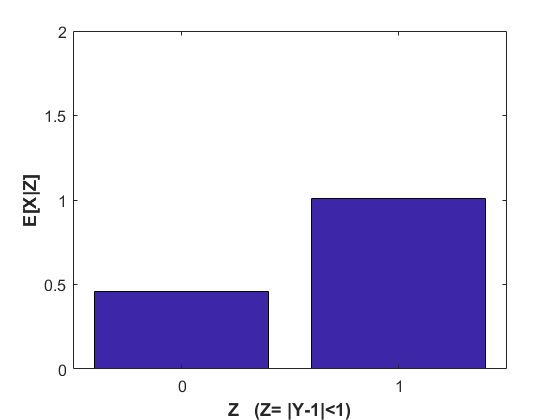
\includegraphics[width=\textwidth]{./Images/2/1.png}
			\caption{ \lr{$E[X|Z]$ vs $Z$ where $Z= |Y-1|<1$ ($0$ for false, $1$ for true)} }
		\end{subfigure}
		\quad
		\begin{subfigure}[h!]{0.8\textwidth}
			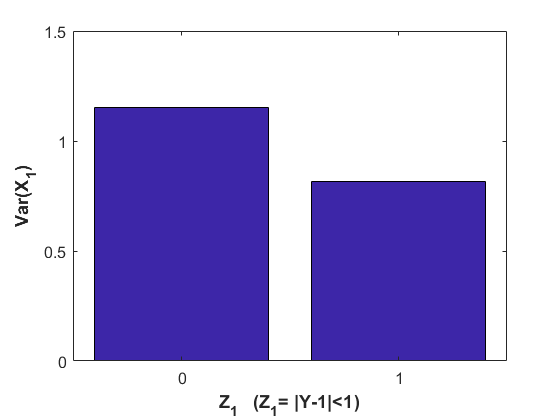
\includegraphics[width=\textwidth]{./Images/2/2.png}
			\caption{ \lr{$Var(X_1)$ vs $Z_1$ where $Z_1=\ |Y-1|<1$ ($0$ for false, $1$ for true)} }
		\end{subfigure}
	\end{figure}
	\begin{figure}[h!]\ContinuedFloat
		\centering
		\begin{subfigure}[h!]{0.8\textwidth}
			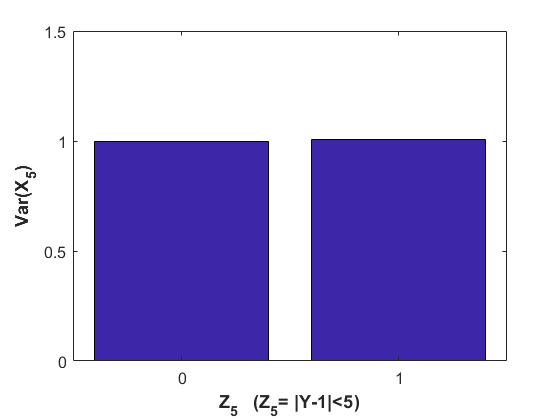
\includegraphics[width=\textwidth]{./Images/2/3.png}
			\caption{ \lr{$Var(X_5)$ vs $Z_5$ where $Z_5=\ |Y-1|<5$ ($0$ for false, $1$ for true)} }
		\end{subfigure}
		\quad
		\begin{subfigure}[h!]{0.8\textwidth}
			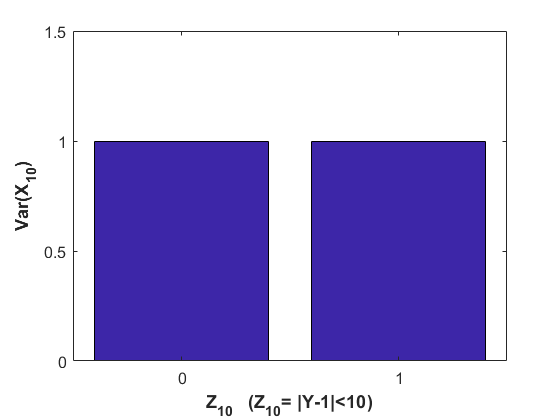
\includegraphics[width=\textwidth]{./Images/2/4.png}
			\caption{ \lr{$Var(X_{10})$ vs $Z_{10}$ where $Z_{10}=\ |Y-1|<10$ ($0$ for false, $1$ for true)} }
		\end{subfigure}
	
		\caption{نمودار‌های پرسش ۲}
		\label{q2}
	\end{figure}
	
	%% 4
	\begin{figure}[h!]
		\centering
		\begin{subfigure}[h!]{0.8\textwidth}
			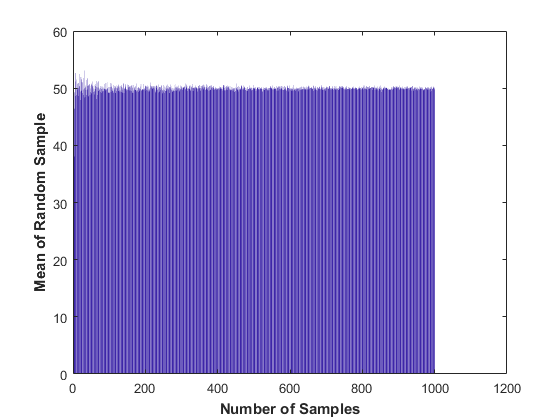
\includegraphics[width=\textwidth]{./Images/4/1.png}
			\caption{ \lr{Random Sample Mean-Sampling x Points} }
		\end{subfigure}
		\quad
		\begin{subfigure}[h!]{0.8\textwidth}
			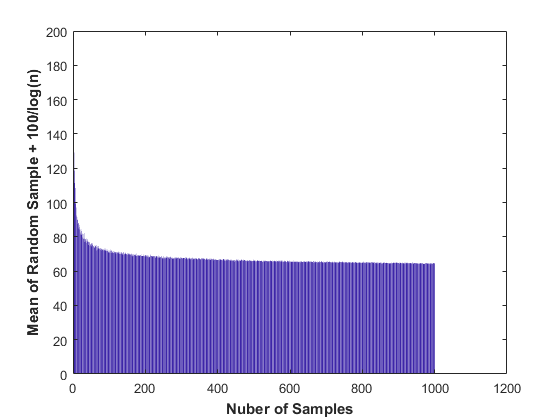
\includegraphics[width=\textwidth]{./Images/4/2.png}
			\caption{ \lr{Random Sample Mean + 100/log(n)-Sampling x Points} }
		\end{subfigure}
		
		\caption{نمودار‌های پرسش ۴}
		\label{q4}
	\end{figure}
	
	%% 5
	\begin{figure}[h!]
		\centering
		\begin{subfigure}[h!]{0.8\textwidth}
			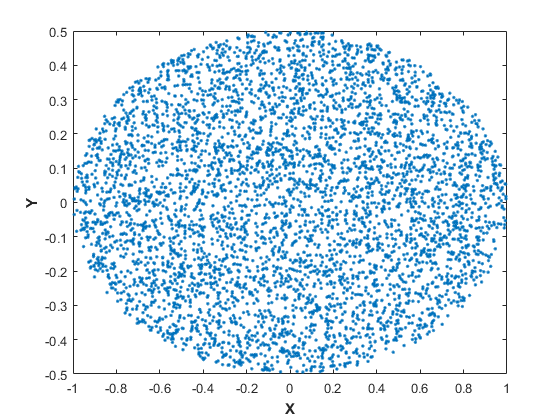
\includegraphics[width=\textwidth]{./Images/5/5000.png}
			\caption{ \lr{$5000$ pseudo-randomly and uniformly selected points in $x^2 + 4y^2 \le 1$.} }
		\end{subfigure}
		\quad
		\begin{subfigure}[h!]{0.8\textwidth}
			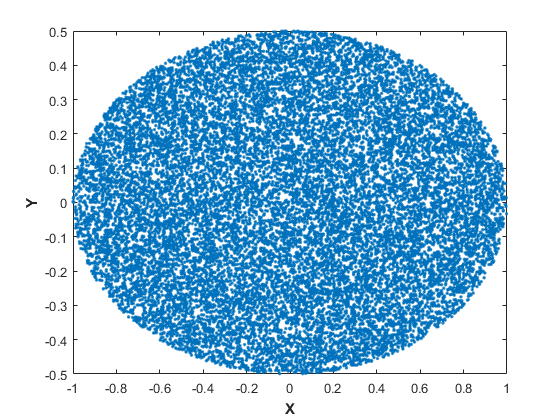
\includegraphics[width=\textwidth]{./Images/5/20000.png}
			\caption{ \lr{$20000$ pseudo-randomly and uniformly selected points in $x^2 + 4y^2 \le 1$.} }
		\end{subfigure}
	\end{figure}
	\begin{figure}[h!]\ContinuedFloat
		\centering
		\begin{subfigure}[h!]{0.8\textwidth}
			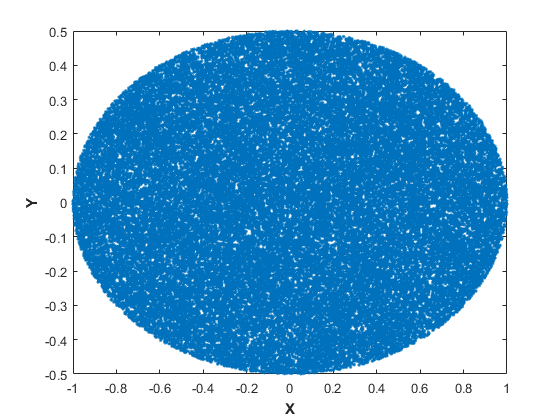
\includegraphics[width=\textwidth]{./Images/5/50000.png}
			\caption{ \lr{$50000$ pseudo-randomly and uniformly selected points in $x^2 + 4y^2 \le 1$.} }
		\end{subfigure}
		\quad
		\begin{subfigure}[h!]{0.8\textwidth}
			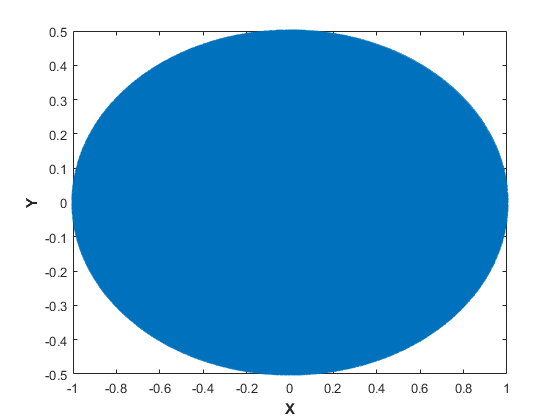
\includegraphics[width=\textwidth]{./Images/5/1000000.png}
			\caption{ \lr{$1000000$ pseudo-randomly and uniformly selected points in $x^2 + 4y^2 \le 1$.} }
		\end{subfigure}
		\caption{نمودار‌های پرسش ۵}
		\label{q5}
	\end{figure}
\end{document}